\subsection{SDL2 GUI implementation}
\label{sec:sdl2gui}

Since we're using SDL2, we've made an implementation of the UIComponent class
 with the following template arguments:
\begin{itemize}
\item T = SDL\_Renderer (Rendering engine used by SDL2)
\item D = sdl\_data (a data structure)
\item R = SDL\_Texture (SDL2's texture structure)
\item S = sdl\_mouse\_event\_data (data used by the mouse callback object)
\end{itemize}

Other components like panels and buttons can inherit from this class and use 
custom data structures that inherit from the sdl\_data struct as shown in 
\cref{fig:sdluicomponent-inherit}.

\begin{figure}[!htb]
\centering
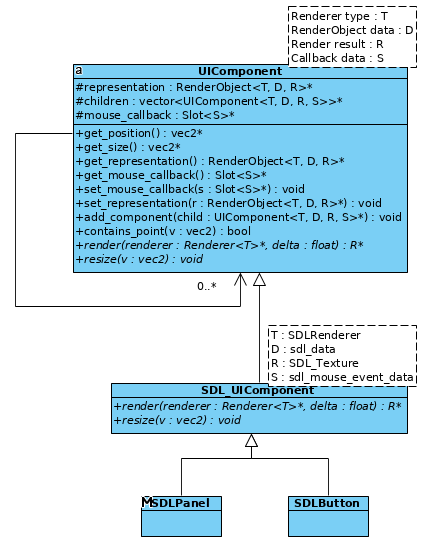
\includegraphics[scale=0.75]{res/ui/sdluicomponent-inherit.png}
\caption{SDL\_UIComponent class inheritance.}\label{fig:sdluicomponent-inherit}
\end{figure}

